\documentclass[conference]{IEEEtran}
\usepackage{cite}
\usepackage{amsmath,amssymb,amsfonts}
\usepackage{algorithmic}
\usepackage{graphicx}
\usepackage{textcomp}
\usepackage{xcolor}
\def\BibTeX{{\rm B\kern-.05em{\sc i\kern-.025em b}\kern-.08em
    T\kern-.1667em\lower.7ex\hbox{E}\kern-.125emX}}
    
\usepackage{float}
\usepackage[caption=false]{subfig}
\usepackage{url,hyperref}

\begin{document}

\title{MoReL: Molecule Representation Learning Toolkit\\
	{
		\footnotesize \textsuperscript{}
	}
		\thanks{}
}

\author{
	\IEEEauthorblockN{
		Songhao Jiang\IEEEauthorrefmark{1}, 
		Xiaotian Duan\IEEEauthorrefmark{2},
	}
	\IEEEauthorblockA{
		\textit{Department of Computer Science} \\
		\textit{The University of Chicago}\\
		Emails: \IEEEauthorrefmark{1}shjiang@uchicago.edu, \IEEEauthorrefmark{2}xduan7@uchicago.edu,
	}
}

\maketitle

\begin{abstract}

There are multiple ways to featurize molecules, and more than a couple of suitable deep learning models for any one of these features. 
Moreover, for each one of the feature and model combination, there are different sets of hyper-parameters to explore. 
The combinatorial number of learning instances to run is in the scale of thousands if not more, which makes it crucial to have a robust and efficient system to help us with data loading, as well as the arrangement and parallelization of the jobs. 
We are planning on implementing a light-weight toolkit, MoRel, for this purpose. 

\end{abstract}

\begin{IEEEkeywords}
deep learning, system, molecule, representation learning
\end{IEEEkeywords}

\section{Introduction} \label{sec_intro} 

The properties of a molecule is at the heart of many problems, from drug synethsis to material discovery. 
With the rising popularity of deep learning and the support of underlying hardwares, more and more efforts have been put into the research of representation learning of molecules using neural networks. 
However, unlike images or natural language corpora, featurizing (transforming into vectors of numbers for statistical learning) molecules is rather unintuitive. 
Thus, different ways of featurization have been invented to incoorperate human understanding of the molecules into learning models, like SMILES (Simplified molecular-input line-entry system) strings, fringerprints \cite{ecfp}, decriptors, and graphs. 

Each of these ditinct molecular features are suitable for a different set of deep learning models. 
For example, SMILES strings (e.g. "C02", "C1CCCCC1"), which are entirely made of ASCII characters, are preferably trained on NLP (natural language processing) models like LSTM \cite{lstm} or Transformer \cite{transformer}. 
Similarly, molecular graph features are usually feed into neural networks that are designed for learning graphs, like GGNN \cite{ggnn} or GCN \cite{gcn}. 

Moreover, for each combination of features and model, we need to experiment with different hyper-parameters, like drop out ratios and optimizers, in order to get better performance. 
A model might behave badly or even unstable using one set of hyper-parameters but beat records using another set. 

To sum things up, the combinatorial number of learning instances is at least in the scale of thousands. 
However, no matter which feature, model, and hyper-parameters we choose, the goal stays the same, that is, learning the meaningful and unique representation of a single molecule. 
This ensures the fairness of comparison across all the combinations, which leads to the motivation of MoReL: to build a light-weight toolkit that efficiently enables the comparison between thousands of instances for molecular representation learning. 
There are a few challenges for this project:
\begin{itemize}
	\item[$\bullet$]  There are about 97 million molecules to train with, which takes up to 500GB after featurization. With such scale, dataloading can easily become the bottleneck for training; 
	\item[$\bullet$]  There are only a limited number of GPUs availble and they are usually meant to be shared between multiple users. How to use them conservatively and efficiently is the core of this project; 
	\item[$\bullet$]  Some learning methods already have their Python scripts. We would like our toolkit to ultilize the existing code with minimal changes. This will not only save a lot work, but also enable MoReL to be used on other projects that requires hyper-parameter optimization with existing training scripts. 
\end{itemize}

The layout of this paper are list as follows: 
section \ref{sec_rw} talks about some previous works that are similar or related to ours; 
section \ref{sec_impl} contains planned implementation details and estimated timeline; 
section \ref{sec_eval} includes some possible methods to evaluate the system, which are subject to change drastically in the future. 

\begin{figure*}[!htb] 
	\subfloat[]{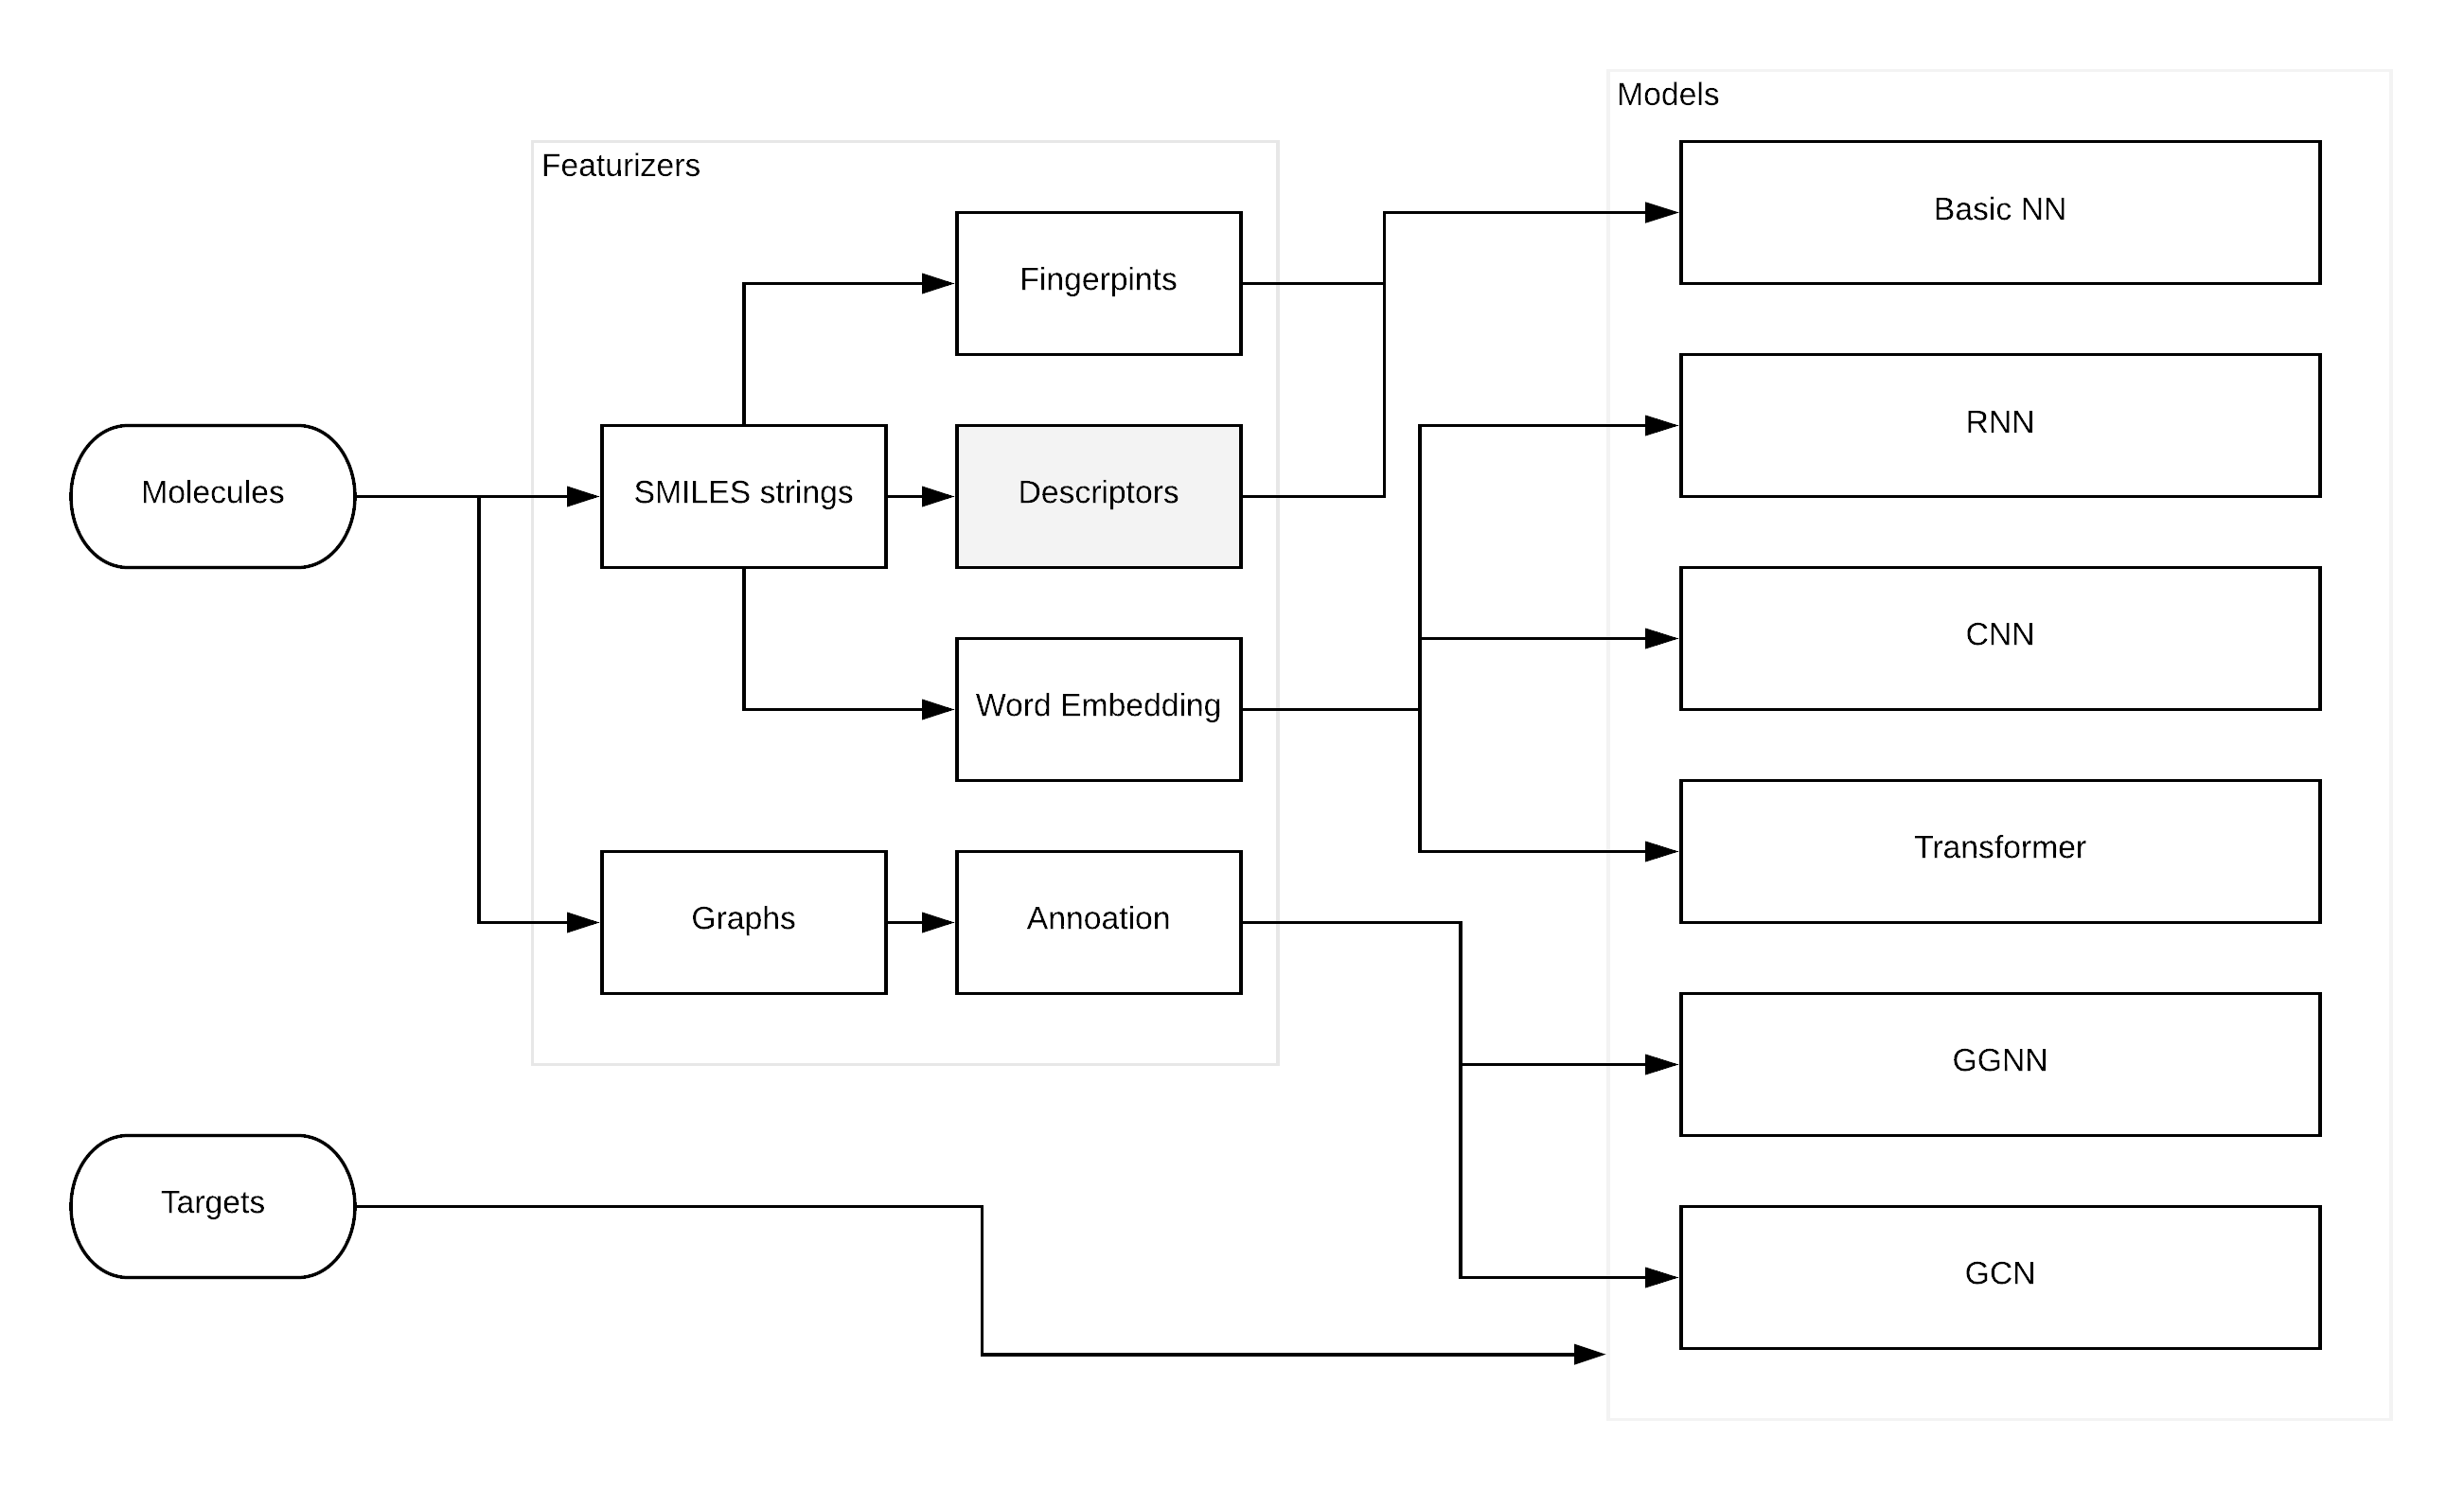
\includegraphics[width=\linewidth]{train.png}}

	\caption{\small 
		Training process flowchart. }
	\label{fig:train}
\end{figure*}

\section{Related Work} \label{sec_rw}

Significant works have been done for the comparison between different methods for molecule represeantion learning. 
For example, \cite{gagcn} has compared the performances with GGNN, GCN, and some variations on molecular learning; \cite{smiles2vec}, \cite{chemception} have tried using SMILES strings and molecular images as features, and tested with some generic models on benchmarked datasets. 
However, the comparison in these works are usually not comprehensive enough to cover a full spectrum of different featurization methods or network structures. 

More similar to our project, MoleculeNet \cite{molnet} is a framework that provides all necessary tools and an environment for comparing a varity of features (fingerpints, graphs, etc.) using different learning algorithms including deep learning, by evaluating performances on benchmarked datasets (HIV, MUV, etc.). 
It serves to offer a ready-to-launch benchark that users can evaluate their models back to back against existing ones. 
Our work differs from MoleculeNet in the following aspects:
\begin{itemize}
	\item[$\bullet$]  MoReL focuses only on deep learning models, with huge amount of training data (around 90 million). MoleculeNet is more inclusive in terms of learning algorithms, but only trained on benchmarked datasets in much smaller scale (less than 500 thousand);
	\item[$\bullet$]  MoReL is designed to train multiple instances in parallel on multiple GPUs, and search for the best combination of features, model, and hyper-parameters. MoleculeNet has no such function;
	\item[$\bullet$]  The implementation of MoReL focus on the efficiency, and can be easily applied to any deep learning project that requires hyper-parameter searching; 
\end{itemize}

\section{Implementation} \label{sec_impl} 

In this section we are going to discuss: \ref{subsec_feas} the feasibility of the project; \ref{subsec_struct} implementation structures in detail; and \ref{sebsec_esttl} estimated timeline and work plan. 

\subsection{Feasibility} \label{subsec_feas} 

For the input data in this project, we are using molecular InChI(The IUPAC International Chemical Identifier) from PubChem, which is directly accessible from PubChem FTP server. 
To extract the training features, RDkit, an open-source cheminformatics software will be used to obtain SMILES strings and fingerpirnts directly from InChI with one-liner APIs. 
As for graph features, there are open-source modules from existing work \cite{gcn_fp} that can be used directly in our project, extracting graph structures from molecules. 
However, there might be some minor changes to be made as our project is much more demanding in performance and efficiency. 

Also, the nerual network implemention is almost half-way done. 
For many models planned in this project, we have individual scripts that takes a set of hyper-parameters as arguments and prints performance evalution after training. 

The most time consuming part in this project is writing a "monitor" program that does the following:
\begin{itemize}
	\item[$\bullet$]  Load and prepare training data;
	\item[$\bullet$]  Arrange jobs to maximize the GPU ultilization;
	\item[$\bullet$]  Save/load/synchronize deep learning jobs; 
\end{itemize}
All these functions are simple and self-explaintory, which justifies the feasibility of this project. 
The motivation and implemenation details of will be wriiten in \ref{subsec_struct}.

In terms of hardware, we have two availble machines for experiment and evaluation. 
One is NVidia DGX statation (256GB RAM, 8TB SSD, 4 GPUs), shared between multiple users; the other one is a high-end PC (32GB RAM, 1TB SSD, 2 GPUs). 

\subsection{Project Structure} \label{subsec_struct}

There are three main components in this projects from development point of view: featurizers, models, and the monitoring process. 
An overall flowchart of featurizers and models in this project is shown in Figure \ref{fig:train}, which highlights the relations between all different kinds of features and models planned in this project. 

The core of this project is a "monitor" process that launches other python scripts that trains and evaluates different models. 
Our major concern is GPU ultilization, which directly correlates to total running time. 
And to achieve higher ultilization, data loading and job arrangement are two closely-related factors. 

\paragraph{Data Loading} 

Considering the estimated scale of features, we cannot fit all features of all molecules in memory, which makes dataloading a potential bottleneck during our training if not handled carefully. 
For example, if there are 4 learning instances running on 4 GPUs separately at the same time, and they are all trying to access different chunks of data stored in SSD, the overhead of dataloading can result in suboptimal GPU ultilization. 

To counter this problem, we have to take advantages of the fact that, there are multiple learning instances using the exact same features (but they are either using different models or running on different hyper-parameters). 
If these instances are trained together in a synchronized fashion, then we only need to load the same small chunk of features at a time. 
This not only reduce the number of SSD accesses, which is a potential bottleneck, but also alleviates redundant feature pre-processing like padding. 
A comparison between the two data loading approaches is shown in Figure \ref{fig:dl}.

\begin{figure}[!htb] 
	\subfloat[Naive implementation of data loading]{%
	  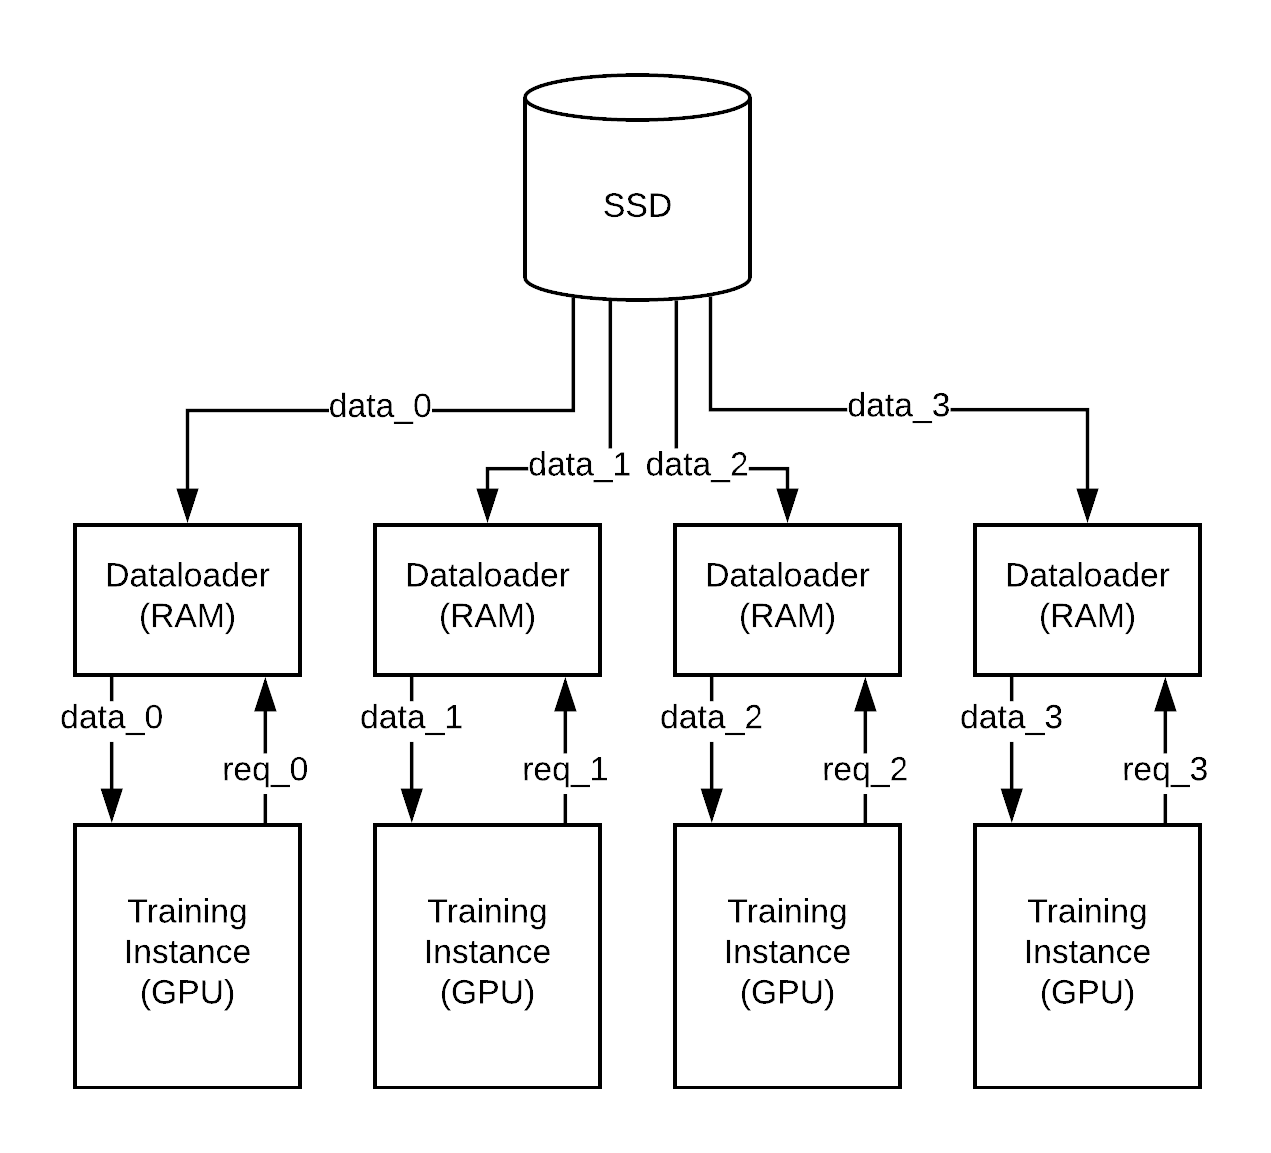
\includegraphics[width=.9\linewidth]{data_loading_a.png} 
	  \label{dl_a} 
	}
	
	\subfloat[Shared data loading]{%
	  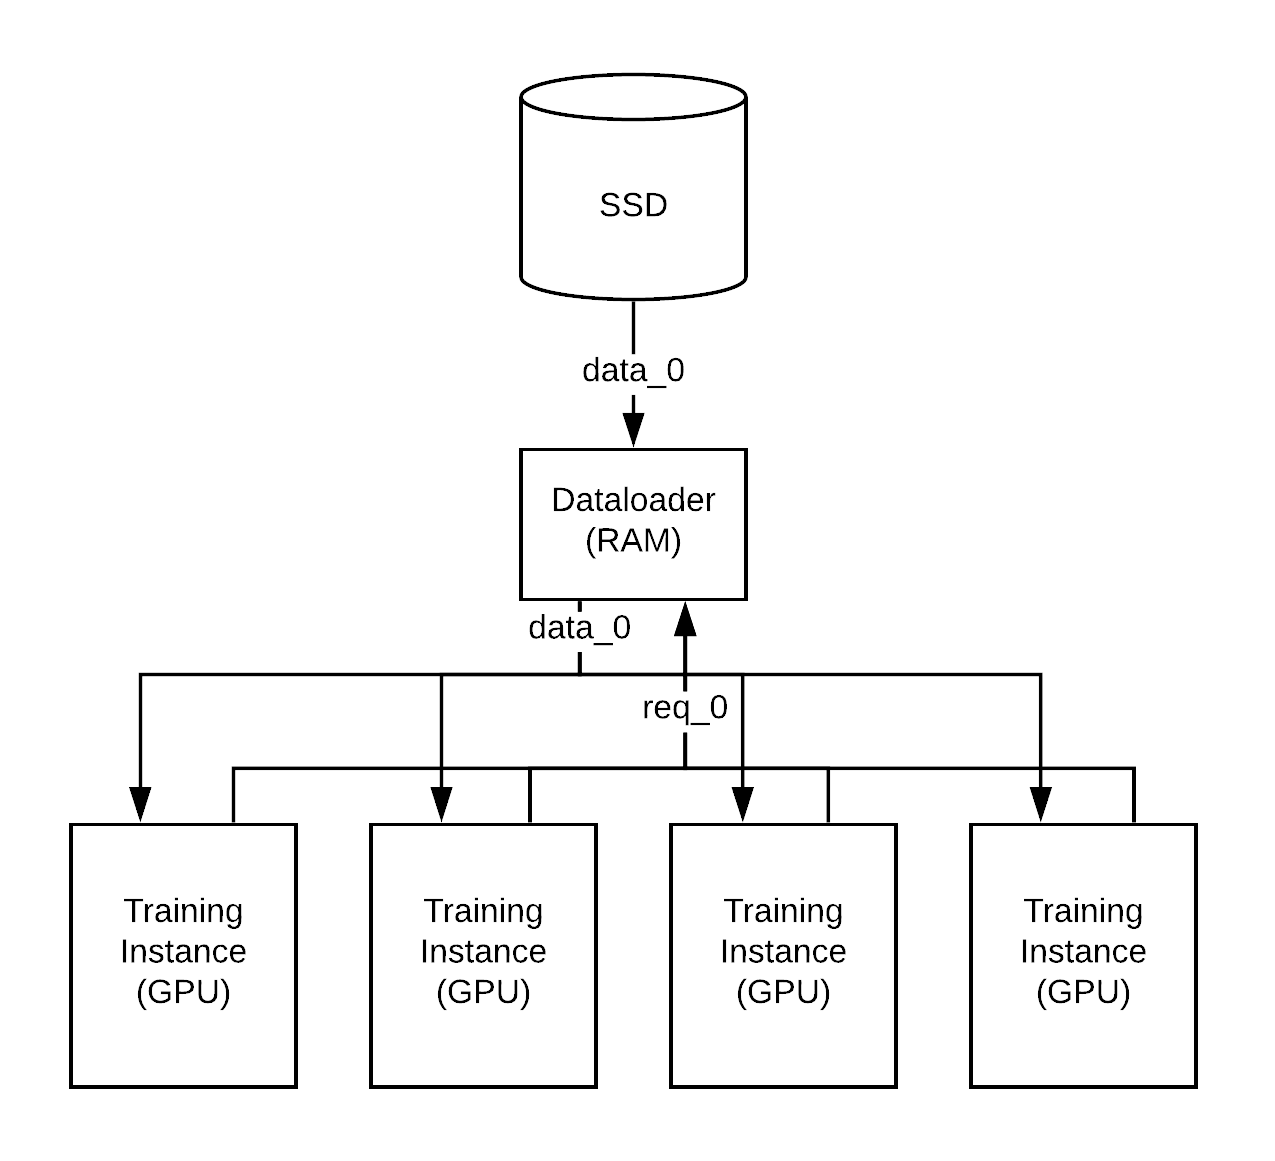
\includegraphics[width=.9\linewidth]{data_loading_b.png} 
	  \label{dl_b} 
	}
	
	\caption{\small 
		Solution \hyperref[dl_a]{(a)}. introduces bottleneck during data retrival from SSD; 
		in \hyperref[dl_b]{(b)}, learning instances sharing the same training data will be executed together to minimize SSD accesses and feature preparation. }
	\label{fig:dl}
\end{figure}

There are two ways to implement such data sharing between different learning instances (python processes): 

\begin{itemize}
	\item[1.]  using off-the-shelf database with in-memory caching;
	\item[2.]  writing a customized pre-fetching dataloader that communicates with learning instances with signal and shares data with mmap;
\end{itemize}

The customized dataloader is indeed more flexible and introduces less overhead. 
But it also tricky to implement with some inter-process-communication and synchronization problems to take care of. 
In this project, we will start with database and see if there is still need for a more efficent dataloader. 
These are the two most straightforward ways that I can come up with at the planning stage. 
There might be better implementation as we move along the project and gain more insights about the system. 

\paragraph{Job Arrangement}
On the other hand, the data sharing approach shown in Figure \ref{fig:dl}\hyperref[dl_b]{(b)} requires training jobs to be executed in a synchronized way, that is, all the instances will fetch the next batch of data at relatively the same time. 
If a GPU has faster training progress than the others, it will have to wait sooner or later (depending on synchronization granularity) to ensure the data sharing is still feasible. 
The synchronization will indeed introduce overhead and lower GPU ultilization, especially if the learning jobs running together have very different training time per batch. 
We are hoping that by putting the jobs with similar number of neurons together, the synchronization overhead will be negligible. 

Note that in most cases, a learning job can be executed on a single GPU. 
By using more than one GPUs for a single job, the speedup is usually significantly lower than the number of GPUs we used. 
And because of the huge combinatorial number of jobs to run, the system can almost always arrange similar jobs to execute together. 

But in some scenarios, we might have a "standout" job that is not suitable for the arrangement:
\begin{itemize}
	\item[$\bullet$]  Last job(s) for a certain kind of features;
	\item[$\bullet$]  A job that has significantly more neurons than the rest;
	\item[$\bullet$]  A job that requires multi-GPU to run properly; 
\end{itemize}
In these cases, the system will parallelize the "standout" jobs to all the GPUs avaible in order to finish it as soon as possible. 
For example, if we only have 2 jobs left, then the system will run each job on dual GPU.

\subsection{Estimated Timeline} \label{sebsec_esttl}

The estimated timeline and milestones are shown in Table \ref{tl_tb}, which are suject to change with implementation progress. 

\begin{table}[!htb]
	\centering
	\caption{\small 
		Estimated timeline. }
	\label{tl_tb}
	\resizebox{0.8\linewidth}{!}{%
	\begin{tabular}{|l|l|}
		\hline
		Time      & Milestone                       \\ \hline
		Feb. 9th  & molecule featurizers            \\ \hline
		Feb. 16th & neural network models           \\ \hline
		Feb. 23rd & all individual learning scripts \\ \hline
		Mar. 2nd  & job arrangement                 \\ \hline
		Mar. 9th  & shared dataloader               \\ \hline
		Mar. 14th & report and presentation         \\ \hline
	\end{tabular}%
	}
\end{table}

\section{Evaluations} \label{sec_eval}

The evaulation of this project can be divided into the following three parts in order:
\begin{itemize}
	\item[$\bullet$]  Fundamentally, MoReL should be running flawlessly on both testing machines with shared hardware resources;
	\item[$\bullet$]  Comparison of the running time between naive/indivudal and shared data loading approaches on idle environment. 
		This will help us indentify whether SSD access becomes a bottleneck during the training. 
		If not, the project still reduces the number of SSD accesses by 75\%, which is meaningful on a resource-sharing machine. 
	\item[$\bullet$]  We expect to see an average GPU ultilization level of at least 80\%. 
		Higher ultilization indicates efficient data loading and job arrangement;
\end{itemize}


\begin{thebibliography}{}
	\bibitem{ecfp} D. Rogers and M. Hahn, “Extended-Connectivity Fingerprints,” Journal of Chemical Information and Modeling, vol. 50, no. 5, pp. 742–754, 2010.
	\bibitem{lstm} S. Hochreiter and J. Schmidhuber, “Long Short-Term Memory,” Neural Computation, vol. 9, no. 8, pp. 1735–1780, 1997.
	\bibitem{transformer} Vaswani, Ashish, Shazeer, Noam, Parmar, Niki, Jakob, Jones, Gomez, A. N., Kaiser, Lukasz, Polosukhin, and Illia, “Attention Is All You Need,” [astro-ph/0005112] A Determination of the Hubble Constant from Cepheid Distances and a Model of the Local Peculiar Velocity Field, 06-Dec-2017. [Online]. Available: https://arxiv.org/abs/1706.03762. [Accessed: 30-Jan-2019].
	\bibitem{ggnn} Li, Yujia, Tarlow, Daniel, Brockschmidt, Marc, Zemel, and Richard, “Gated Graph Sequence Neural Networks,” [astro-ph/0005112] A Determination of the Hubble Constant from Cepheid Distances and a Model of the Local Peculiar Velocity Field, 22-Sep-2017. [Online]. Available: https://arxiv.org/abs/1511.05493. [Accessed: 30-Jan-2019].
	\bibitem{gcn} T. N. and Max, “Semi-Supervised Classification with Graph Convolutional Networks,” [astro-ph/0005112] A Determination of the Hubble Constant from Cepheid Distances and a Model of the Local Peculiar Velocity Field, 22-Feb-2017. [Online]. Available: https://arxiv.org/abs/1609.02907. [Accessed: 30-Jan-2019].
	\bibitem{gagcn} Ryu, Seongok, Lim, Jaechang, S. Hwan, Kim, and W. Youn, “Deeply learning molecular structure-property relationships using attention- and gate-augmented graph convolutional network,” [astro-ph/0005112] A Determination of the Hubble Constant from Cepheid Distances and a Model of the Local Peculiar Velocity Field, 08-Oct-2018. [Online]. Available: https://arxiv.org/abs/1805.10988. [Accessed: 30-Jan-2019].
	\bibitem{smiles2vec} Goh, G. B., Hodas, N. O., Siegel, Charles, and Abhinav, “SMILES2Vec: An Interpretable General-Purpose Deep Neural Network for Predicting Chemical Properties,” [astro-ph/0005112] A Determination of the Hubble Constant from Cepheid Distances and a Model of the Local Peculiar Velocity Field, 18-Mar-2018. [Online]. Available: https://arxiv.org/abs/1712.02034. [Accessed: 30-Jan-2019].
	\bibitem{chemception} Goh, Garrett, Siegel, Charles, Abhinav, Hodas, N. O., Baker, and Nathan, “Chemception: A Deep Neural Network with Minimal Chemistry Knowledge Matches the Performance of Expert-developed QSAR/QSPR Models,” [astro-ph/0005112] A Determination of the Hubble Constant from Cepheid Distances and a Model of the Local Peculiar Velocity Field, 20-Jun-2017. [Online]. Available: https://arxiv.org/abs/1706.06689. [Accessed: 30-Jan-2019].
	\bibitem{molnet} Wu, Bharath, Feinberg, E. N., Gomes, Joseph, Geniesse, Caleb, Pappu, Karl, and Vijay, “MoleculeNet: A Benchmark for Molecular Machine Learning,” [astro-ph/0005112] A Determination of the Hubble Constant from Cepheid Distances and a Model of the Local Peculiar Velocity Field, 26-Oct-2018. [Online]. Available: https://arxiv.org/abs/1703.00564. [Accessed: 30-Jan-2019].
	\bibitem{gcn_fp} David, Maclaurin, Jorge, Gómez-Bombarelli, Rafael, Hirzel, Alán, Adams, and R. P., “Convolutional Networks on Graphs for Learning Molecular Fingerprints,” [astro-ph/0005112] A Determination of the Hubble Constant from Cepheid Distances and a Model of the Local Peculiar Velocity Field, 03-Nov-2015. [Online]. Available: https://arxiv.org/abs/1509.09292. [Accessed: 30-Jan-2019].
\end{thebibliography}


\end{document}
